%!TEX root = ../these.tex

\section{
  Визуализация геометрической информации
}
\label{sec:json.view}

На разных этапах
как научных исследований,
так и технологической подготовки производства,
возникает потребность визуализации разнообразной
геометрической информации,
такой как геометрия деталей
и ограничивающих их контуров,
положение допустимых точек врезки
и выключения инструмента,
маршруты,
получаемые в ходе
решения различных классов задач резки,
а также маршруты движения резака,
получаемые после обработки постпроцессором
и т.п.

Традиционным подходом к визуализации является
разработка специализированных графических утилит
либо отдельных графических представлений
в рамках больших программных систем.
Зачастую этот подход является оправданным,
но у него есть и свои недостатки ---
прежде всего усложнение процесса разработки
и тестирования программного обеспечения.
Кроме того,
полученные таким образом визуализации
могут использоваться,
например, для научных публикаций,
только посредством создания растровых копий экранов,
или же требуется разработка отдельной функциональности
для экспорта визуализации в файл некоторого формата.

Альтернативный подход,
зачастую оказывающийся
\textit{гораздо}
легче в разработке,
заключается в том,
чтобы визуализация производилась
путём экспорта в некоторый графический формат,
который уже может широко использоваться как
для распространения,
так и для собственно просмотра при помощи
стандартных утилит.
Стандартом де-факто в наше время
для этой цели является формат
SVG~\cite{bi:SVG},
а для его оперативного отображения
может использоваться любой современный браузер,
впрочем как и множество готовых библиотек
для встраивания в разрабатываемое программное обеспечение.
Важным достоинством такого подхода
является его кросс-платформенность,
то есть возможность использовать его
на большинстве платформ и операционных систем.

В данной диссертационной работе
как раз повсеместно и использовался формат SVG
при намеренном отказе от разработки
собственных программ визуализации.
Например,
в Листинге~\ref{lst:json-svg}
приводится простейший SVG-файл,
сгенерированный для раскройной карты,
представленной на Листинге~\ref{lst:json-dbs}.

\lstinputlisting[
  language=XML,
  basicstyle=\footnotesize,
  showstringspaces=false,
  numbers=left,
  label={lst:json-svg},
  captionpos=b,
  caption=SVG-файл для визуализации раскроя из Листинга~\ref{lst:json-dbs}
  ]
  {media/nesting.svg}

Можно заметить,
что команды SVG
практически идеально соответствуют
элементам геометрической информации.
Фактически,
SVG может использоваться даже
как альтернативный вариант
хранения и обмена графической информацией
(вместо DXF, DBS, JSON\dots),
хотя в данной работе этого не происходило,
утилиты раздела~\ref{sec:json-dbs.js}
только экспортируют в SVG
без возможности обратного преобразования.

\subsection{Настройка параметров визуализации}

Значительный объем работы при реализации
специализированных утилит для визуализации
составляет подбор параметров изображения,
таких как цвета объектов, размеры линий
и т.п.
Как правило требуется предоставить пользователю
возможность влиять на такие решения,
что дополнительно усложняет и сам программный код
и взаимодействие с ним пользователя.

Формат SVG
в свою очередь глубоко интегрирован с механизмом
каскадных таблиц стилей
(Cascading Style Sheets, CSS),
также являющимся современным
активно развивающимся стандартом.
Благодаря этому получается
упростить вопросы настройки параметров визуализации.
Фактически,
речь идёт о редактировании одного или нескольких
текстовых файлов,
а возможности CSS очень велики~\cite{bi:CSS}
и в общем превосходят
потребности CAD/CAM-систем:
\begin{itemize}
  \item Настройка цветов изображений.
  \item Настройка толщин, цветов и вида линий.
  \item Настройка заливки фигур,
  включая сплошную, градиентную
  и штриховую,
  что необходимо для CAD-систем.
  \item Широкие возможности геометрических трансформаций
  всего изображения или групп объектов,
  включая сдвиг, поворот, отражение и масштабирование.
  \item Построение теней
  \item Возможность анимации,
  как постоянно действующей,
  так и интерактивной
  \item И многое другое\dots
\end{itemize}

\begin{figure}
  \centering
  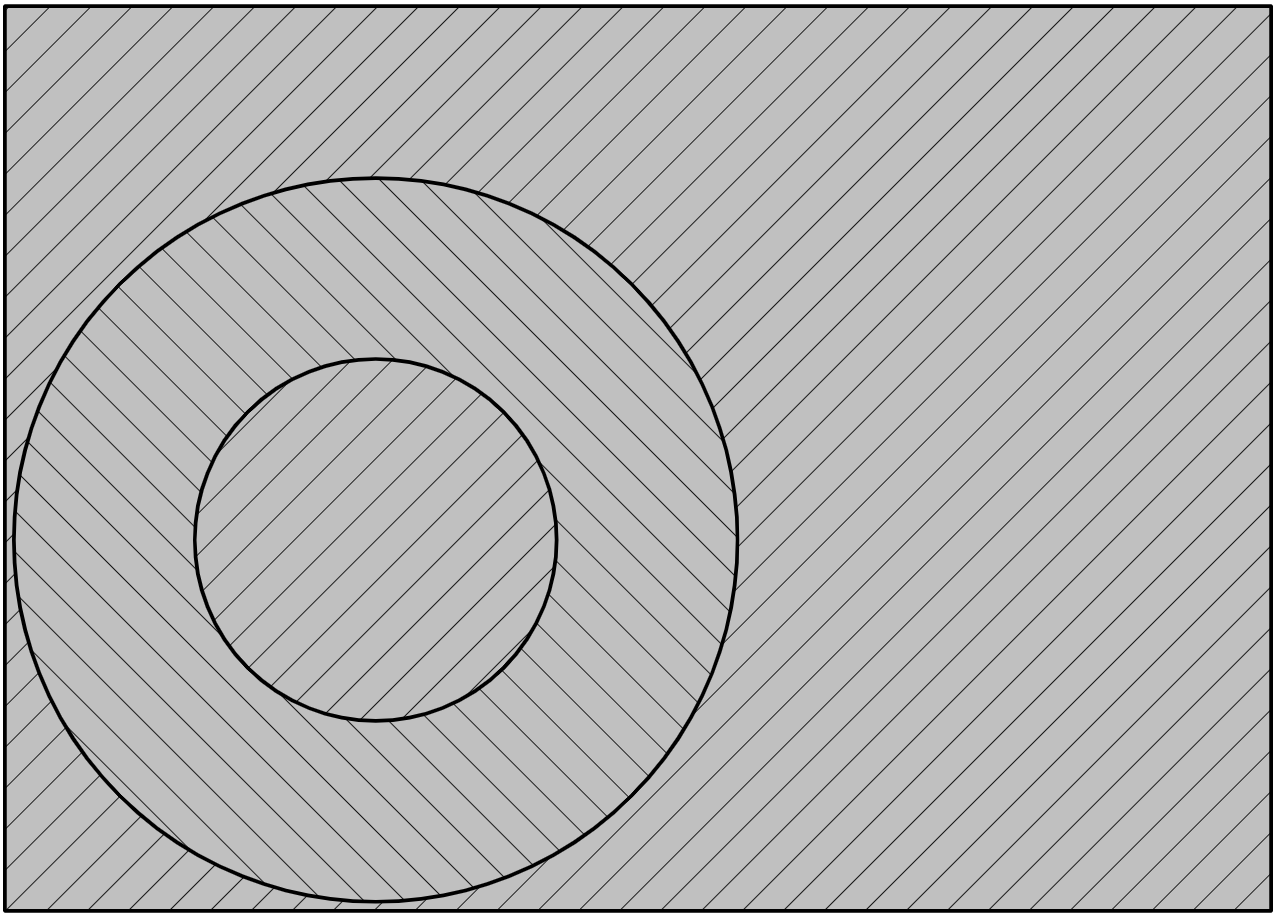
\includegraphics[width=0.5\textwidth]{nesting.png}
  \caption{Визуализация раскроя из Листинга~\ref{lst:json-dbs}}
  \label{fig:json-nesting}
\end{figure}

В ходе данной диссертационной работы
были разработаны несколько схем
оформления получаемых SVG-файлов,
интегрированные в утилиты раздела~\ref{sec:json-dbs.js}.
Один из вариантов оформления
SVG-файла из Листинга~\ref{lst:json-svg}
приведён на рис.~\ref{fig:json-nesting}.

\subsection{Организация пользовательского интерфейса}

Когда визуализация представлена на мониторе,
у пользователя зачастую возникает потребность
взаимодействия с изображением ---
как целиком,
например, изменить масштаб,
повернуть или подвинуть его на экране,
так и с отдельными его элементами,
например, навести на него курсор мыши
и получить дополнительную информацию,
удалить, сдвинуть или изменить его
и т.п.
Удобная организация графического
пользовательского интерфейса
(GUI)
традиционно является одной из сложных
задач программирования.
Кроме того,
именно в этой области
чаще всего возникают сложности
с переносимостью программного кода
между разными платформами и операционными системами.

Использование SVG
и здесь позволяет использовать
огромный опыт,
накопленный в области организации пользовательского интерфейса
за десятилетия развития Web-технологий.
Объекты SVG
широко поддерживают управление при помощи языка
JavaScript~\cite{bi:JavaScript},
также являющегося главным
(а до недавнего времени --- единственным)
языком программирования,
исполняемым в браузерах.

Программы на языке JavaScript
способны реагировать на огромное количество событий,
включая сюда
\begin{itemize}
  \item нажатие пользователем клавиш на клавиатуре
  \item движение курсора мыши
  \item нажатие кнопок мыши
  \item события таймера
  \item загрузку страницы и завершение ее просмотра
  \item начало и конец анимации объектов
\end{itemize}
и производить с объектами страницы произвольные действия:
\begin{itemize}
  \item прятать их и восстанавливать
  \item создавать новые объекты и удалять их
  \item двигать, увеличивать или уменьшать
  \item изменять цвета, шрифты, способы заливки
  \item изменять текст
\end{itemize}
и многое другое.
Благодаря этому возможна организация сколь угодно
сложных сценариев взаимодействия с пользователем.

При этом нет необходимости разрабатывать все это самостоятельно,
целиком, <<с нуля>>.
В мире создано и регулярно создается
огромное количество библиотек и фреймворков,
реализующих разные аспекты пользовательского интерфейса
на высоком уровне абстракции.
Например,
утилиты раздела~\ref{sec:json-dbs.js}
для организации
масштабирования и прокрутки
встраивают в экспортируемый SVG-файл
обращение к внешней
библиотеке с открытым кодом
svg-pan-zoom~\cite{bi:svg-pan-zoom}.

Для визуализации решения задачи PCGTSP
(см. Главу~\ref{ch:pcgtsp}),
которая требует объединения
информации,
полученной из нескольких источников
(раскройная карта;
координаты допустимых точек врезки;
индексы вершин оптимального маршрута),
была разработана специализированная утилита
\cite{bi:j2pcgtsp}.

Для разработки использовался стек технологий,
сходный с описанным в разделе~\ref{sec:json-dbs.js}:
язык JavaScript~\cite{bi:JavaScript}
и его диалект
LiveScript~\cite{bi:LiveScript},
система сборки rollup.js~\cite{bi:rollup.js}.
Утилита изначально являлась кросс-платформенной.
Сначала она разрабатывалась
как утилита командной строки,
но опыт использования в данном исследовании
показал,
что это неудобно,
и она была трансформирована в Web-приложение
Single Page Application
(SPA),
которое может запускаться в браузере,
как локально,
так и будучи размещенным на произвольном хостинге.

Пример созданного ею изображения
оптимального решения задачи PCGTSP
для
34 кластеров
приведен на рис.~\ref{fig:pcgtsp.svg},
стр.~\pageref{fig:pcgtsp.svg}.
